
\title{Recap Database Management System (01NVVOV)}
\author{Jacopo Nasi\\
        Computer Engineer\\
        Politecnico di Torino}
\date{I Period - 2017/2018\\\bigskip\bigskip\today}

\documentclass[12pt]{article}
\usepackage[utf8]{inputenc}
\usepackage[italian]{babel}
\usepackage{geometry}
\usepackage{indentfirst} % First line indent
\usepackage{mathtools}
\usepackage{wrapfig}
\usepackage[usenames, dvipsnames]{color}
\usepackage{float}
\usepackage{amssymb}
\usepackage{ifsym}
% Misure Documento
\geometry{ a4paper, total={170mm,257mm},left=35mm, right=35mm, top=35mm, bottom=35mm }

\begin{document}

\begin{figure}
  \centering
  
\includegraphics[width=10cm]{images/polito.pdf}
\end{figure}

\maketitle

\newpage
\tableofcontents

\newpage
{\noindent \Large \textbf{License}\bigskip}

This work is licensed under a Creative Commons Attribution-NonCommercial-ShareAlike 3.0 Unported License.\\
You are free:
\begin{itemize}
  \item \textbf{to Share}: to copy, distribute and transmit the work
  \item \textbf{to Remix}: to adapt the work
\end{itemize}
Under the following conditions:
\begin{itemize}
  \item \textbf{Attribution}: you must attribute the work in the manner specified by the author or licensor (but not in any way that suggests that they endorse you or your use of the work)
  \item \textbf{Noncommercial}: you may not use this work for commercial purposes.
  \item \textbf{Share Alike}: if you alter, transform, or build upon this work, you may distribute the resulting work only under the same or similar license to this one.
\end{itemize}

\noindent More information on the Creative Commons website (http://creativecommons.org).

\begin{figure}[h!]
  \centering
  
\includegraphics[width=3cm]{images/license.png}
\end{figure}

{\noindent \Large \textbf{Acknowledgments}\bigskip}

Questo breve riepilogo non ha alcuno scopo se non quello di agevolare lo studio di me stesso, se vi fosse di aiuto siete liberi di usarlo.\\
Le fonti su cui mi sono basato sono quelle relative al corso offerto (\textbf{Database Management System (01NVVOV)}) dal Politecnico di Torino durante l'anno accademico 2017/2018.\\
Non mi assumo nessuna responsabilità in merito ad errori o qualsiasi altra cosa. Fatene buon uso!
\newpage

\section{Database Management System}
\subsection{Introduction}

The DataBase Management System \textbf{DBMS} is a software package designed to store and manage databases. The architecture of the system is similar to the one in the figure \ref{fig:arch}.
\begin{figure}[h!]
  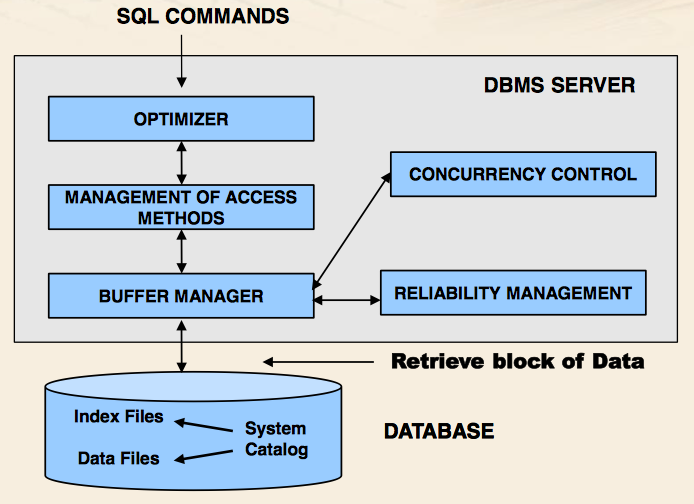
\includegraphics[width=\linewidth]{images/arch.png}
  \caption{DBMS Architecture}
  \label{fig:arch}
\end{figure}
Since the DB data part can be really big it can't fit always in the main memory (RAM) and, for this fact, is often stored in the secondary memory, like HDD. For this reason is necessary a system that define the operations to grab and manage the data from the secondary memory.\\
All the blocks has different behaviours. The \textbf{Optimizer} have multiple roles:
\begin{itemize}
  \item Define an appropriate execution strategy for accessing data to answer queries.
  \item Receives in input the SQL instructions (DML).
  \item Check the lexical, syntactical and sematical correctness (not all the errors).
  \item Translate the query in an internal algebra rappresentation.
  \item Select the "right" strategy for accesing data.
  \item Guarantees the \textbf{data independence} property in the relation model.
\end{itemize}
The \textbf{Access Method Manager} is used for physical access to data and it implements the strategy selected by the optimizer. The \textbf{Buffer Manager} instead manage the page transfert from disk to main memory and vice versa and the main memory portion that is pre-allocated to the DBMS that is shared among many applications. The \textbf{Concurrency Control} coordinate the concurrent access to data (important for write operations) to guarantess the consistency of it. The \textbf{Realiability Manager} guarantees correctness of the database content duing the system crashes, the atomic execution of a transaction and it exploits auxiliary structures (log files) the correct the database in case of failure.\\
The \textbf{transaction} is an unit of work performed by an application, it's a sequence of one or more SQL RW operation charaterized by \textit{correctness, reliability} and \textit{isolation}. The START of a transaction is typically implicit and coincides with the first SQL instruction. The END instead can be of two differents types, it can be a COMMIT that it means the correct end of a transaction, or with ROLLBACK that it means error during the execution. In this second case the DBMS needs to go back to the state at the beginning of the transaction. The rollback can be of two type suicide, when is required by the transaction, and murder when is required by the system. The transaction have four important properties:
\begin{itemize}
  \item \textbf{A}tomicity
  \item \textbf{C}onsistency
  \item \textbf{I}solation
  \item \textbf{D}urability
\end{itemize}
Atomicity means that they cannot be divided in smaller units, is not possibile to leave the system in a intermediate state of exec, guarantee by UNDO (undoes all the work perfomed, used for rollback) and REDO (redoes all work performed, used for commit the result in presence of failure). The consistency means that the transaction execution should not violate integrity constraints on a database, in case of it the system will perform solution to correct the violation. The system can be considered Isolated when the execution of a transaction is indipendent of the concurrent execution of other transaction, everything is enforced by the Concurrency Control block. The last properties means that, in presence of failures, the effect of a commited transaction IS NOT LOST, it guarantees the reliability of the DBMS and is enforced by the Reliability Manager block. % 3/9/17 @ 18:15

\bibliographystyle{abbrv}
\bibliography{simple}

\end{document}
